\section{Theoretischer Hintergrund}
\subsection{Einleitung}
Mit Hilfe des spezifischen Widerstandes lässt sich der ohmsche Widerstand von homogenen geometrischen Formen sehr einfach berechnen. Das Ziel dieses Versuches ist die Bestimmung der Dicke einer Aluminiumfolie.
Dieser Versuch hat folgende Zielsetzungen: Rechnen mit SI - Einheiten, Bedienen von Messgeräten in der Gleichstromlehre, Anwenden von Strom- und Spannungsfehlerschaltung, Anwenden der 4-Leiter Messung, Abschätzen der Grenzen von Modellen und Vereinfachungen.
\subsection{Vorbereitung}
Kreieren Sie Ihren eigen persönlichen Widerstand, indem Sie Aluminiumfolie auf einen Karton kleben und ein längliches Rechteck herausschneiden. Fertigen Sie mindestens zwei davon an.
\begin{center}
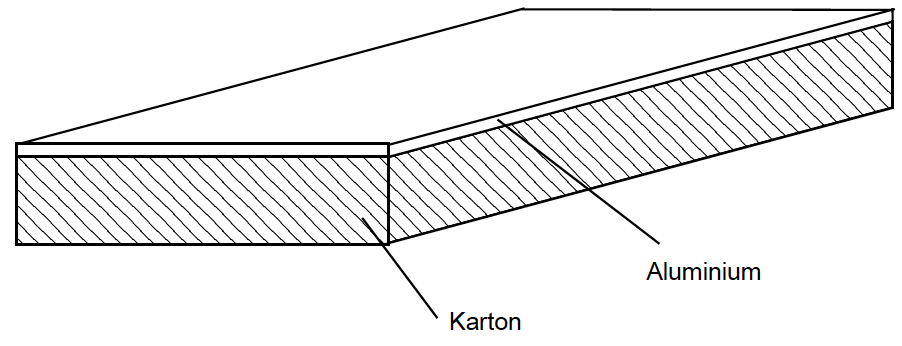
\includegraphics[scale=0.5]{../img/II/IIa}
\end{center}
\subsection{Das Ohmsche Gesetz}
Das Ohmsche Gesetz beschreibt den Zusammenhang von Strom und Spannung bei einem ohmschen Widerstand. Bei einem Widerstand von $1\Omega$ fliesst bei einer Spannung von $1\text{V}$ ein Strom von $1\text{A}$.
\begin{equation}
\boxed{R=\dfrac{U}{I},\quad \begin{array}{l}R:\text{ohmscher Widerstand} \text{ [}\Omega\text{]}\\U:\text{Spannung} \text{ [V]}\\I:\text{Strom}\text{ [A]}\end{array}}
\end{equation}
\subsection{Die Leistung im Gleichstromkreis}
Bei Gleichspannung gilt
\begin{equation}
\boxed{\begin{array}{lll}P&=&U\cdot I\\P&=&I^2\cdot R\\P&=&\dfrac{U^2}{R}\end{array},\quad [P]=\text{Watt}=\text{V}\cdot \text{A}}
\end{equation}
Allgemein für nicht konstante Werte ist die Leistung
\begin{equation}
\boxed{P=\dfrac{1}{T}\displaystyle \int_0^Tp\left(t\right)\text{d}t=\dfrac{1}{T}\displaystyle \int_0^Tu\left(t\right)\cdot i\left(t\right)\text{d}t}
\end{equation}
\subsection{Der spezifische Widerstand}
Mit Hilfe des spezifischen Widerstandes lässt sich der ohmsche Widerstand eines homogenen Körpers berechnen.
\begin{equation}
\boxed{R=\dfrac{\rho\cdot l}{A}=\dfrac{l}{\sigma\cdot A}}
\end{equation}
wobei $R$ der ohmsche Widerstand in $\Omega$, $\rho$ der spezifische Widerstand in $\Omega\text{m}$, $l$ die Länge des Körpers in $\text{m}$, $A$ die Querschnittsfläche in $\text{m}^2$ und $\sigma$ die Leitfähigkeit in $\Omega^{-1}\text{m}^{-1}$.
\begin{center}
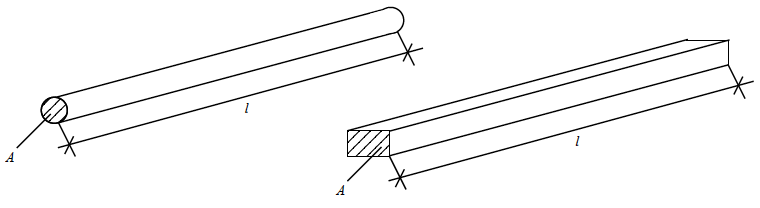
\includegraphics[scale=0.5]{../img/II/IIb}
\end{center}
\subsection{Die Spannungsfehlerschaltung}
\begin{center}
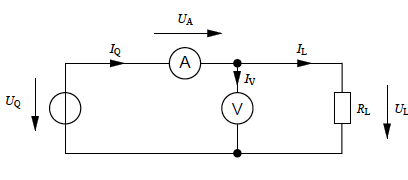
\includegraphics[scale=1]{../img/II/IId}
\end{center}
Bei der Spannungsfehlerschaltung entsteht ein \textbf{Spannungsteiler} aus dem Innenwiderstand des Strommessgerätes und dem zu messenden Widerstand. Der \textbf{Spannungsabfall} $U_A$ am Strommessgerät verfälscht die Spannungsmessung. Die gemessene Spannung $U_Q$ ist um die Spannung $U_A$ zu gross.
\\\\
Folgende Messung wurde mit $R=10\Omega$ gemacht
\begin{center}
\begin{tabular}{cccc}\hline
$U/\text{V}$&$I/\text{A}$&$R/\Omega$ (Spannungsfehler)&$R/\Omega$ (Stromfehler)\\\hline
20&2,4&10000&8333\\
0,2&0,024&10000&8333\\\hline
\end{tabular}
\end{center}
Typischerweise ist der Innenwiderstand von Strommessern \textbf{sehr klein}. Die Spannungsfehlerschaltung eignet sich deshalb nur für Messungen an \textbf{grossen Widerständen}, wo der Spannungsabfall am Innenwiderstand des Strommessers die Messung sehr wenig beeinflusst. Sobald man mit dieser Schaltung einen kleinen Widerstand messen will, verfälscht die Reihenschaltung aus Innenwiderstand des Strommessers und dem zu messenden Widerstand das Ergebnis.
\\\\
Die Spannungsfehlerschaltung wird bei hochohmigen Lastwiderständen $\boxed{R_L>1\text{M}\Omega}$ gebraucht.
\subsection{Die Stromfehlerschaltung}
\begin{center}
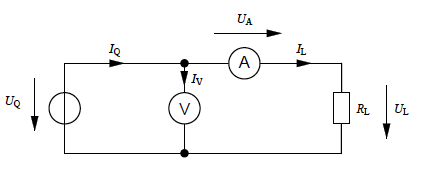
\includegraphics[scale=1]{../img/II/IIc}
\end{center}
Bei der Stromfehlerschaltung besteht eine \textbf{Parallelschaltung} aus dem Innenwiderstand des Spannungsmessers und dem zu messenden Widerstand. Durch den Spannungsmesser fliesst ein Strom $I_V$. Dieser verfälscht den zu messenden Strom $I_L=U_L/R_L$, der durch den zu messenden Widerstand fliesst. Der Strom $I_Q$ ist um den Strom $I_L$, der durch den Spannungsmesser fliesst, zu gross.
\\\\
Folgende Messung wurde mit $R=220\Omega$ gemacht.
\begin{center}
\begin{tabular}{cccc}\hline
$U/\text{V}$&$I/\text{A}$&$R/\Omega$ (Spannungsfehler)&$R/\Omega$ (Stromfehler)\\\hline
20&90&222&222\\
0,2&0,91&333&220\\\hline
\end{tabular}
\end{center}
Typischerweise ist der Innenwiderstand von Spannungsmessern \textbf{sehr gross}. Die Stromfehlerschaltung eignet sich deshalb nur zur Widerstandsmessung an \textbf{kleinen Widerständen}, wo der Strom durch den Innenwiderstand des Spannungsmessers, die Messung sehr wenig beeinflusst. Sobald man mit dieser Schaltung an einem grossen Widerstand messen will, verfälscht die Parallelschaltung aus Innenwiderstand des Spannungsmessers und dem zu messenden Widerstand das Ergebnis.
\\\\
Die Stromfehlerschaltung wird bei niederohmigen Lastwiderständen $\boxed{1\Omega<R_L<1\text{M}\Omega}$ gebraucht.
\subsection{Multimeter}
Elektronische Multimeter sind bei der Spannungsmessung \textbf{sehr hochohmig} (1..10\text{M}$\Omega$). Daher hat die Stromfehlerschaltung nur dann eine Bedeutung wenn sehr kleine Ströme ($\mu$A-Bereich) gemessen werden. Die Spannungsfehlerschaltung kommt aber ebenso zur Anwendung, weil der Shunt-Widerstand im Messgerät einen relevanten Spannungsabfall bewirkt.
\subsection{Die 4-Leiter Messung}
Bei sehr \textbf{niederohmigen Widerstandsmessungen} bevorzugt man die 4-Leiter Messung. Die 4-Leiter Messung ist eine Erweiterung der Stromfehlerschaltung. Die Spannung wird aber direkt über der Last gemessen. So wird der Spannungsabfall über den Zuleitungen nicht mitgemessen.
\begin{center}
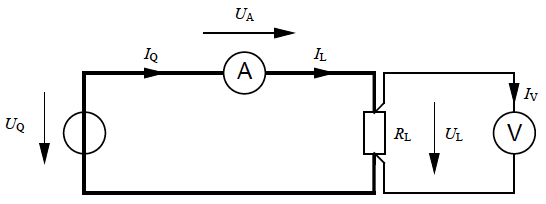
\includegraphics[scale=0.8]{../img/II/IIe}
\end{center}
\section{Versuchsanleitung}
\subsection{Theoretische Aufgaben}
\begin{enumerate}[$a)$]
\item Berechnen Sie den \textbf{ohmschen Widerstand} einer Stromschiene aus Kupfer mit einer rechteckigen Querschnittsfläche von 3cm auf 10 cm. Die Länge beträgt 52 Meter.
{\color{red}{\begin{equation*}
\begin{array}{lll}
R&=&\dfrac{l}{\sigma_{Cu}\cdot A}\\
&=&\dfrac{52\text{m}}{\left(5.7\cdot 10^{7}\Omega^{-1}\text{m}^{-1}\right)\cdot \left(3\cdot 10^{-2}\text{m}\right)\cdot \left(10\cdot 10^{-2}\text{m}\right)}\\
&=&3.04\cdot 10^{-4}\Omega\\
\end{array}
\end{equation*}}}
\item Leiten Sie die Leistungsformel her
{\color{red}{\begin{equation*}
\begin{array}{lll}
P&=&U\cdot I=\left(R\cdot I\right)\cdot I=R\cdot I^2\\
&=&U\cdot I=U\cdot \left(\dfrac{U}{R}\right)=\dfrac{U^2}{R}
\end{array}
\end{equation*}}}
\item Die vielfach verwendeten bedrahteten Widerstände (Metallfilmwiderstände) haben eine maximale Belastbarkeit von 0.6 Watt. Berechnen sie die \textbf{maximalen Ströme} für einen $1\Omega$, $1k\Omega$ und einen $10k\Omega$ Widerstand. Berechnen Sie für die gleichen Widerstände, die \textbf{maximal zulässige Spannung}. Kann es für einen Widerstand andere Einschränkungen für die maximale Spannung geben, als die maximal zulässige Leistung?
{\color{red}{\begin{center}
\begin{tabular}{cc|cc}\hline
$P/\text{Watt}$&$R/\Omega$&$I_{\text{max}}$/\text{A}&$U_{\text{max}}/\text{V}$\\\hline
$6\cdot 10^{-1}$&$1$&$7.7\cdot 10^{-1}$&$7.7\cdot 10^{-1}$\\
$6\cdot 10^{-1}$&$1\cdot 10^{3}$&$2.4\cdot 10^{-2}$&$24.5$\\
$6\cdot 10^{-1}$&$1\cdot 10^{4}$&$7.7\cdot 10^{-3}$&$77.5$\\
\hline
\end{tabular}
\end{center}}}
\begin{equation}
\boxed{I_{\text{max}}=\sqrt{\dfrac{P}{R}}}\quad \boxed{U_{\text{max}}=\sqrt{P\cdot R}}
\end{equation}
\item Berechnen sie allgemein die Dicke der Aluminiumfolie, wenn Sie den ohmschen Widerstand und die Geometrie kennen.
{\color{red}{\begin{equation*}
R=\dfrac{\rho\cdot l}{A}=\dfrac{\rho\cdot l}{b\cdot d}\Rightarrow d=\dfrac{\rho\cdot l}{b\cdot R}=\dfrac{l}{\sigma\cdot b\cdot R}
\end{equation*}}}
\item In der Literatur wird häufig der spezifische Widerstand in [$\Omega\text{mm}^2\text{m}^{-1}$] angegeben. Bestimmen Sie den Umrechnungsfaktor um den spezifischen Widerstand in [$\Omega\text{m}$] angeben zu können.
{\color{red}{\begin{equation*}
\Omega\text{m}=\Omega\text{mm}^2\text{m}^{-1}\cdot \dfrac{1\text{m}^2}{\left(1000\text{mm}\right)^2}\Rightarrow \text{Faktor}=\dfrac{1}{10^{6}}
\end{equation*}}}
\item Welche Schaltungsart (Ohmmeter, Spannungsfehlerschaltung, Stromfehlerschaltung, 4-Leiter Messung) ist wohl die genauste für die Widerstandsbestimmung der Aluminiumfolie?
\\\\
{\color{red}{$\Rightarrow$ Die 4-Leiter-Messung.}}
\item Sie bestimmen einen elektrischen Widerstand durch Strom- und Spannungsmessung mit der \textbf{Stromfehlerschaltung}. Der Lastwiderstand beträgt ungefähr $1\text{M}\Omega$, der Innenwiderstand des Voltmeters ca. $20\text{M}\Omega$. Schätzen sie den Fehler ab, wenn Sie davon ausgehen, dass die Messgeräte selber keinen Fehler aufweisen. Berechnen Sie den Fehler genau.
{\color{red}{\begin{equation*}
R_L=1\cdot 10^{6}\Omega,\quad R_V=20\cdot 10^6\Omega\Rightarrow \dfrac{1}{20}=0.2=20\%
\end{equation*}}}
\item Überlegen Sie sich, wo die Grenzen der Formel des \textbf{spezifischen Widerstandes} liegen resp. welche Annahmen bei dieser Formel getroffen werden.
\\\\
{\color{red}{$\Rightarrow$ Materialtoleranzen.}}
\end{enumerate}
\subsection{Dicke der Aluminiumfolie in Längsrichtung}
Benutzen Sie Ihre selbstgebauten Widerstände nur in \textbf{Längsrichtung}.
\subsubsection{Ohmmeter}
\textbf{Messerwartung:}
\\
\textbf{Messaufbau:}
\\
\textbf{Messresultate:}
\\
\textbf{Diskussion:}
\subsubsection{Spannungsfehlerschaltung}
\textbf{Messerwartung:}
\\
\textbf{Messaufbau:}
\\
\textbf{Messresultate:}
\\
\textbf{Diskussion:}
\subsubsection{Stromfehlerschaltung}
\textbf{Messerwartung:}
\\
\textbf{Messaufbau:}
\\
\textbf{Messresultate:}
\\
\textbf{Diskussion:}
\subsubsection{4-Leiter Messung}
\textbf{Messerwartung:}
\\
\textbf{Messaufbau:}
\\
\textbf{Messresultate:}
\\
\textbf{Diskussion:}
\subsection{Dicke der Aluminiumfolie in Querrichtung}
Benutzen Sie Ihre selbstgebauten Widerstände nur in \textbf{Querrichtung}.
\subsubsection{Ohmmeter}
\textbf{Messerwartung:}
\\
\textbf{Messaufbau:}
\\
\textbf{Messresultate:}
\\
\textbf{Diskussion:}
\subsubsection{Spannungsfehlerschaltung}
\textbf{Messerwartung:}
\\
\textbf{Messaufbau:}
\\
\textbf{Messresultate:}
\\
\textbf{Diskussion:}
\subsubsection{Stromfehlerschaltung}
\textbf{Messerwartung:}
\\
\textbf{Messaufbau:}
\\
\textbf{Messresultate:}
\\
\textbf{Diskussion:}
\subsubsection{4-Leiter Messung}
\textbf{Messerwartung:}
\\
\textbf{Messaufbau:}
\\
\textbf{Messresultate:}
\\
\textbf{Diskussion:}
\section{Leitfähigkeiten}
\begin{center}
\begin{tabular}{ccc}\hline
\textbf{Material}&\textbf{Typ}&\textbf{$\sigma$ / $\Omega^{-1}\text{m}^{-1}$}\\\hline
Quarz &Isolator&$\approx 10^{-17}$\\
Silikonöl&Isolator&$\approx 10^{-15}$\\
Mica&Isolator&$\approx 10^{-15}$\\
Paraffin&Isolator&$\approx 10^{-15}$\\
Hartgummi &Isolator&$\approx 10^{-15}$\\
Porzellan&Isolator&$\approx 10^{-14}$\\
Glas&Isolator&$\approx 10^{-12}$\\
Bakelit&Isolator&$\approx 10^{-9}$\\
Destilliertes Wasser&Isolator&$\approx 10^{-4}$\\
Sandige Erde, trocken &schlechter Isolator&$\approx 10^{-3}$\\
Feuchte Erde &schlechter Isolator&$\approx 10^{-2}$\\
Frischwasser &schlechter Isolator&$\approx 10^{-2}$\\
Tierisches Fett&schlechter Isolator&$\approx 4\cdot 10^{-2}$\\
Tierischer Muskel &schlechter Leiter&$0.4$\\
Tierisches Blut &schlechter Leiter&$0.7$\\
Germanium (rein)&Halbleiter&$\approx 2$\\
Meerwasser &Leiter&$\approx 4$\\
Tellur&Leiter&$\approx 5\cdot 10^{2}$\\
Kohle &Leiter&$\approx 3\cdot 10^{4}$\\
Graphit &Leiter&$\approx 10^{5}$\\
Gusseisen &Leiter&$\approx 10^{6}$\\
Quecksilber &Leiter&$\approx 10^{6}$\\
Chromnickel&Leiter&$\approx 10^{6}$\\
Konstantan &Leiter&$\approx 2\cdot 10^{6}$\\
Blei&Leiter&$\approx 5\cdot 10^{6}$\\
Zinn &Leiter&$\approx 9\cdot 10^{6}$\\
Bronze &Leiter&$\approx 10^{7}$\\
Messing &Leiter&$\approx 1.1\cdot 10^{7}$\\
Zink &Leiter&$\approx 1.7\cdot 10^{7}$\\
Wolfram&Leiter&$\approx 1.8\cdot 10^{7}$\\
Aluminium &Leiter&$\approx 3.0\cdot 10^{7}$\\
Aluminium hartgezogen &Leiter&$\approx 3.5\cdot 10^{7}$\\
Gold&Leiter&$\approx 4.5\cdot 10^{7}$\\
Kupfer &Leiter&$\approx 5.7\cdot 10^{7}$\\
Silber&Leiter&$\approx 6.1\cdot 10^{7}$\\
Nb3(Al-Ge)&Supraleiter&$\infty$\\\hline
\end{tabular}
\end{center}